\documentclass[11pt,a4paper]{article}

\usepackage[utf8]{inputenc}
\usepackage[T1]{fontenc}
\usepackage[spanish]{babel}
\usepackage{geometry}
\usepackage{graphicx}
\usepackage{array}
\usepackage{tabularx}
\usepackage{makecell}
\usepackage[table]{xcolor}
\usepackage{fancyhdr}
\usepackage{titlesec}
\usepackage{helvet}
\usepackage{ragged2e}
\usepackage{enumitem}
\usepackage{setspace}
\usepackage{hyperref}
\usepackage{booktabs} % Para tablas con acabado profesional
\usepackage{alltt}    % Bloque monoespaciado que si admite macros (lambda, mu, rho)
\usepackage{amsmath}  % Para las formulas del modelo
\usepackage{float}      % habilita [H] (posición exacta)
\usepackage{placeins}   % habilita \FloatBarrier
\raggedbottom           % evita que LaTeX estire el espacio vertical

\renewcommand{\familydefault}{\sfdefault}
\geometry{
  a4paper,
  left=3.0cm,
  right=3.0cm,
  top=2.35cm,
  bottom=2.35cm,
  headheight=1.9cm,
  headsep=0.45cm
}

\setlength{\parindent}{0pt}
\setlength{\parskip}{0.22em}
\setlength{\emergencystretch}{2em}   % evita desbordes de linea en texto justificado
\setlength{\tabcolsep}{6pt}
\renewcommand{\arraystretch}{1.08}

\pagestyle{fancy}
\fancyhf{}
\fancyhead[L]{
\includegraphics[height=1.35cm]{assets/reporte_tecnico_overleaf_logo.png}}
\fancyhead[R]{\vspace{0.1cm}\small FEIRNNR - Carrera de Computación}
\renewcommand{\headrulewidth}{0.5pt}
\renewcommand{\footrulewidth}{0pt}
\makeatletter
\renewcommand{\headrule}{%
  {\color{gray!65}\hrule width\headwidth height\headrulewidth \vskip-\headrulewidth}%
}
\makeatother

\titleformat{\section}
  {\bfseries\fontsize{15}{17}\selectfont}
  {\thesection.}{0.8em}{}
\titlespacing*{\section}{0pt}{0.7ex}{0.2ex}

\newcolumntype{L}[1]{>{\RaggedRight\arraybackslash}p{#1}}
\newcolumntype{Y}{>{\RaggedRight\arraybackslash}X}

% Marca visible de lo que el equipo todavia debe escribir.
\newcommand{\pendiente}[1]{\textcolor{red}{\textbf{[PENDIENTE: #1]}}}

% Paleta de las tablas de la plantilla institucional.
\definecolor{headerblue}{RGB}{19, 93, 126}
\definecolor{rowlight}{RGB}{205, 235, 248}
\definecolor{borderblue}{RGB}{64, 160, 206}

% babel-espanol renombra \tablename como "Cuadro"; el texto usa "Tabla".
\addto\captionsspanish{\renewcommand{\tablename}{Tabla}}

\begin{document}
\thispagestyle{fancy}

\vspace*{0.15cm}

\begin{center}
{\bfseries\fontsize{23}{26}\selectfont
Reporte Técnico de Actividades\\
Práctico-Experimentales Nro. 003\par}
\end{center}

\section{Datos de Identificación del Estudiante y la Práctica}

\noindent
\begin{tabularx}{\textwidth}{|L{0.43\textwidth}|Y|}
\hline
\textbf{Nombre del estudiante(s)} & Jaime Alejandro Landazuri Roman \\ \hline
\textbf{Asignatura} & Simulación \\ \hline
\textbf{Ciclo} & 5 A \\ \hline
\textbf{Unidad} & 1 \\ \hline
\textbf{Resultado de aprendizaje de la unidad} & R1. Aplica análisis estadísticos de los datos
de la Simulación para mejorar la calidad de los resultados, bajo los principios de solidaridad, transparencia, responsabilidad y honestidad. \\ \hline
\textbf{Práctica Nro.} & 003 \\ \hline
\textbf{Título de la Práctica} & Simulación de un sistema de líneas de espera M/M/1 mediante SimPy \\ \hline
\textbf{Nombre del Docente} & José O. Guamán Q. \\ \hline
\textbf{Fecha} & 15 de Octubre de 2026 \\
 & 16 de Octubre 2026 \\ \hline
\textbf{Horario} & Jueves 10h30 a 11h30 \\
 & Viernes 07h30 a 09h30 \\ \hline
\textbf{Lugar} & Aula \\ \hline
\textbf{Tiempo planificado en el Sílabo} & 3 horas \\ \hline
\end{tabularx}

\section{Objetivo(s) de la Práctica}
Simular un sistema de líneas de espera M/M/1 utilizando Python y SimPy, analizando
el comportamiento de los clientes, la cola y el servidor.
\begin{enumerate}
    \item Implementar un modelo M/M/1 utilizando la biblioteca SimPy.
    \item Calcular las principales métricas teóricas del sistema de espera.
    \item Comparar los resultados teóricos con los obtenidos mediante la simulación.
\end{enumerate}

\section{Materiales y reactivos}
\begin{itemize}
    \item Python 3.x (se ejecutó con Python 3.14.8).
    \item Biblioteca SimPy (se ejecutó con SimPy 4.1.2).
    \item NumPy (2.5.4).
    \item Matplotlib (3.11.2).
    \item Editor de código: Visual Studio Code, PyCharm o Jupyter Notebook.
\end{itemize}

\section{Equipos y herramientas}
\begin{itemize}
    \item Computador.
    \item Procesador de 2 núcleos o superior.
    \item Mínimo 4 GB de RAM.
    \item Sistema operativo Linux o macOS.
\end{itemize}

\section{Link Repositorio}
\url{https://github.com/C-ael/Simulacion_Portafolio}

\section{Procedimiento / Metodología Ejecutada}

\subsection{Fundamento teórico}

El modelo \textbf{M/M/1} representa un sistema de líneas de espera con llegadas de
clientes siguiendo una distribución de Poisson, tiempos de servicio con distribución
exponencial, un único servidor y atención de clientes bajo el principio FIFO
(\emph{primero en llegar, primero en ser atendido}).

El modelo utiliza dos parámetros principales:
\begin{itemize}
    \item $\lambda$: tasa promedio de llegada de clientes.
    \item $\mu$: tasa promedio de servicio del servidor.
\end{itemize}

La utilización del servidor se calcula mediante:
\[
\rho = \frac{\lambda}{\mu}
\]

\noindent\textbf{Observación sobre la guía.} La guía de la práctica imprime
$\rho = \mu/\lambda$, lo que contradice su propia condición de estabilidad
$\lambda < \mu$ enunciada unas líneas más abajo y también su pseudocódigo, que usa
$\rho = \lambda/\mu$. Con la fórmula impresa, los tres escenarios de la guía darían
$\rho = 1{,}50$, $1{,}20$ y $1{,}03$, es decir un servidor saturado en los tres casos, y
las medidas $L$, $L_q$, $W$ y $W_q$ no existirían, porque solo están definidas para
$\rho < 1$. Este trabajo usa la definición correcta $\rho = \lambda/\mu$, que es la que
emplea el pseudocódigo de la propia guía y la que aparece en la bibliografía de teoría
de colas.

Para que el sistema sea estable debe cumplirse:
\[
\lambda < \mu
\]

Las principales medidas teóricas del sistema son:

\[
L = \frac{\lambda}{\mu-\lambda} \qquad
L_q = \frac{\lambda^2}{\mu(\mu-\lambda)}
\]

\[
W = \frac{1}{\mu-\lambda} \qquad
W_q = \frac{\lambda}{\mu(\mu-\lambda)}
\]

\begin{table}[h!]
\centering
\setlength{\arrayrulewidth}{0.75pt}
\arrayrulecolor{borderblue}
\renewcommand{\arraystretch}{1.25}
\begin{tabular}{|l|l|}
\hline
\rowcolor{headerblue}
\textbf{\textcolor{white}{Símbolo}} & \textbf{\textcolor{white}{Significado}} \\ \hline
$\lambda$ & Tasa de llegada de clientes \\ \hline
\rowcolor{rowlight}
$\mu$ & Tasa de servicio \\ \hline
$\rho$ & Utilización del servidor \\ \hline
\rowcolor{rowlight}
$L$ & Número promedio de clientes en el sistema \\ \hline
$L_q$ & Número promedio de clientes en la cola \\ \hline
\rowcolor{rowlight}
$W$ & Tiempo promedio en el sistema \\ \hline
$W_q$ & Tiempo promedio de espera en la cola \\ \hline
\end{tabular}
\caption{Notación empleada.}
\end{table}

\subsection{Escenarios ejecutados}

Se ejecutaron los tres escenarios indicados por la guía, todos con $\mu = 3{,}0$:

\begin{table}[h!]
\centering
\setlength{\arrayrulewidth}{0.75pt}
\arrayrulecolor{borderblue}
\renewcommand{\arraystretch}{1.25}
\begin{tabular}{|c|c|c|l|}
\hline
\rowcolor{headerblue}
\textbf{\textcolor{white}{Escenario}} & \textbf{\textcolor{white}{$\lambda$}} & \textbf{\textcolor{white}{$\mu$}} & \textbf{\textcolor{white}{Condición}} \\ \hline
1 & 2{,}0 & 3{,}0 & Sistema estable \\ \hline
\rowcolor{rowlight}
2 & 2{,}5 & 3{,}0 & Mayor utilización \\ \hline
3 & 2{,}9 & 3{,}0 & Cerca de saturación \\ \hline
\end{tabular}
\caption{Escenarios de la guía. La utilización teórica resulta $\rho = 0{,}667$,
$0{,}833$ y $0{,}967$ respectivamente.}
\end{table}

\subsection{Arquitectura e implementación}

El programa se desarrolló en Python siguiendo el pseudocódigo de la guía y se
estructuró en tres capas (modelo, vista y controlador) para que cada medida tuviera un
único responsable en el código. Los componentes son:

\begin{itemize}
    \item \textbf{Escenarios} (\path{modelo/escenarios.py}): cada escenario es un
    objeto con su $\lambda$, su $\mu$ y su condición. Para cambiar un escenario se
    editan sus números y para agregar uno nuevo se añade a la lista \texttt{ESCENARIOS}.
    \item \textbf{Métricas teóricas} (\path{modelo/teoria.py}): calcula $\rho$, $L$,
    $L_q$, $W$ y $W_q$ con las fórmulas del apartado anterior y expone
    \texttt{es\_estable()} para verificar $\lambda < \mu$. Sus valores son los que se
    comparan con los de la simulación.
    \item \textbf{Motor de simulación} (\path{modelo/simulacion.py}): crea un entorno
    SimPy con un servidor de \texttt{capacity = 1} y genera los clientes con tiempos
    entre llegadas exponenciales de tasa $\lambda$ (\texttt{expovariate}). Cada cliente
    pide el servidor, espera su turno en orden FIFO y es atendido con un tiempo
    exponencial de tasa $\mu$. Por cada cliente se registra el tiempo de espera en cola,
    y aparte se guarda una traza del tamaño de la cola a lo largo del tiempo.
    \item \textbf{Tablas} (\path{vista/tabla.py}): imprime en la terminal la tabla de
    valores teóricos y la tabla de teoría contra simulación. No calcula nada.
    \item \textbf{Gráficas} (\path{vista/graficas.py}): genera las tres figuras del
    informe y las guarda en \texttt{graficas/}.
    \item \textbf{Controlador} (\path{controlador/controlador.py}): recorre los
    escenarios, simula cada uno varias veces, promedia las réplicas y une el modelo con
    la vista. Si un escenario no cumple $\lambda < \mu$, avisa que el sistema no es
    estable, no lo simula y continúa con el siguiente.
    \item \textbf{Punto de entrada} (\path{main.py}): un solo comando ejecuta todo el
    estudio:
\end{itemize}

\begin{verbatim}
python3 main.py
\end{verbatim}

\noindent\textbf{Medición de las métricas simuladas.} Dos detalles de implementación
importan para que los números sean comparables con la teoría:

\begin{itemize}
    \item La \textbf{espera promedio} se calcula como el promedio simple de los tiempos
    de espera de todos los clientes atendidos en la corrida. Mientras más clientes se
    atienden, más se acerca a $W_q$, aunque al empezar con el sistema vacío tiende a
    quedar un poco por debajo.
    \item El \textbf{tamaño promedio de la cola} no se calcula como el promedio simple
    de los tamaños registrados, porque cada tamaño dura un tiempo distinto y eso
    distorsionaría el resultado. Se calcula como el \emph{promedio ponderado por
    tiempo}: cada tamaño de cola se multiplica por el tiempo que permaneció en ese valor
    y al final se divide entre el tiempo total simulado. Así se obtiene $L_q$ de forma
    comparable con la teoría.
\end{itemize}

\noindent\textbf{Sistemas no estables.} Si en algún escenario $\lambda \geq \mu$ el
programa no simula: informa que el sistema no es estable y sigue con los demás. Esto
respeta el pseudocódigo de la guía y evita reportar promedios de una cola que crece sin
límite.

\subsection{Parámetros de la corrida oficial y reproducibilidad}

La corrida que alimenta este informe se ejecutó con la configuración definida en el
controlador, en el archivo \path{controlador/controlador.py}:

\begin{table}[h!]
\centering
\setlength{\arrayrulewidth}{0.75pt}
\arrayrulecolor{borderblue}
\renewcommand{\arraystretch}{1.25}
\begin{tabular}{|l|c|l|}
\hline
\rowcolor{headerblue}
\textbf{\textcolor{white}{Variable}} & \textbf{\textcolor{white}{Valor}} & \textbf{\textcolor{white}{Qué controla}} \\ \hline
\texttt{TIEMPO\_SIMULACION} & 5000 & Duración de cada corrida, en unidades de tiempo \\ \hline
\rowcolor{rowlight}
\texttt{REPETICIONES} & 10 & Réplicas independientes por escenario \\ \hline
\texttt{SEMILLA} & 42 & Semilla base; la réplica $i$ usa \texttt{SEMILLA + i} \\ \hline
\end{tabular}
\caption{Parámetros de la corrida oficial.}
\end{table}

En total se ejecutaron \textbf{30 simulaciones}: 3 escenarios $\times$ 10 réplicas. La
corrida es \textbf{reproducible}: como cada réplica recibe una semilla derivada de forma
determinista de la semilla base, repetir \texttt{python3 main.py} produce exactamente
los mismos números. En cada corrida se atendieron del orden de $10\,000$ clientes en el
escenario 1, $12\,500$ en el escenario 2 y $14\,400$ en el escenario 3.

\section{Resultados esperados}
\begin{itemize}
    \item Un sistema M/M/1 funcional mediante SimPy.
    \item Simulación de llegada de clientes y atención por un único servidor.
    \item Tiempo promedio de espera de los clientes.
    \item Tamaño promedio de la cola.
    \item Utilización teórica del servidor.
    \item Valores teóricos de $L$, $L_q$, $W$ y $W_q$.
    \item Gráficas del comportamiento de la cola y los tiempos de espera.
    \item Comparación entre resultados teóricos y simulados.
    \item Análisis del comportamiento del sistema para los tres escenarios propuestos.
\end{itemize}

\noindent La guía anticipa que \emph{se espera observar que, cuando $\lambda$ se
aproxima a $\mu$, aumentan el tiempo de espera y el tamaño de la cola, debido a que el
servidor trabaja cerca de su capacidad máxima}. Los resultados de la sección siguiente
registran esas medidas; su interpretación va en el análisis de resultados.

\section{Resultados}

\subsection{Comparación entre resultados teóricos y simulados}

La Tabla~\ref{tab:comparacion} presenta, para cada escenario, los valores teóricos
obtenidos con las fórmulas del modelo y los valores simulados obtenidos como promedio
de las 10 réplicas.

\begin{table}[h!]
\centering
\setlength{\arrayrulewidth}{0.75pt}
\arrayrulecolor{borderblue}
\renewcommand{\arraystretch}{1.3}
\small
\begin{tabular}{|c|c|c|c|c|c|c|c|c|}
\hline
\rowcolor{headerblue}
\textbf{\textcolor{white}{Esc.}} &
\textbf{\textcolor{white}{$\lambda$}} &
\textbf{\textcolor{white}{$\rho$}} &
\textbf{\textcolor{white}{$L$}} &
\textbf{\textcolor{white}{$L_q$}} &
\textbf{\textcolor{white}{$W$}} &
\textbf{\textcolor{white}{$W_q$}} &
\makecell{\textbf{\textcolor{white}{Espera}} \\ \textbf{\textcolor{white}{simulada}}} &
\makecell{\textbf{\textcolor{white}{Cola}} \\ \textbf{\textcolor{white}{simulada}}} \\ \hline
1 & 2{,}0 & 0{,}6667 & 2{,}0000 & 1{,}3333 & 1{,}0000 & 0{,}6667 & \textbf{0{,}6691} & \textbf{1{,}3350} \\ \hline
\rowcolor{rowlight}
2 & 2{,}5 & 0{,}8333 & 5{,}0000 & 4{,}1667 & 2{,}0000 & 1{,}6667 & \textbf{1{,}8141} & \textbf{4{,}5500} \\ \hline
3 & 2{,}9 & 0{,}9667 & 29{,}0000 & 28{,}0333 & 10{,}0000 & 9{,}6667 & \textbf{8{,}5730} & \textbf{24{,}8003} \\ \hline
\end{tabular}
\caption{Comparación de resultados teóricos y simulados por escenario. Las columnas
$\rho$, $L$, $L_q$, $W$ y $W_q$ son teóricas; las dos últimas son los promedios
simulados de 10 réplicas.}
\label{tab:comparacion}
\end{table}

Los mismos valores son los que imprime el programa en la terminal al ejecutar
\texttt{python3 main.py}:

\begin{alltt}\small
=== Valores teóricos ===
Escenario          \(\lambda\)     \(\mu\)        \(\rho\)        L       Lq        W       Wq
Escenario 1      2.0   3.0    0.667    2.000    1.333    1.000    0.667
Escenario 2      2.5   3.0    0.833    5.000    4.167    2.000    1.667
Escenario 3      2.9   3.0    0.967   29.000   28.033   10.000    9.667

=== Teoría vs simulación ===
Escenario       Wq teórico  Wq simulado   Dif %   Lq teórico  Lq simulado   Dif %
Escenario 1          0.667        0.669     0.4        1.333        1.335     0.1
Escenario 2          1.667        1.814     8.8        4.167        4.550     9.2
Escenario 3          9.667        8.573   -11.3       28.033       24.800   -11.5
\end{alltt}

\subsection{Intervalo de confianza y error relativo}

La Tabla~\ref{tab:intervalos} reporta, para las dos medidas que produce la simulación
($W_q$ y $L_q$), la media de las 10 réplicas, su desviación estándar, el intervalo de
confianza al 95\,\% y el error relativo frente al valor teórico. El intervalo se calculó
con la distribución $t$ de Student sobre las 10 medias por réplica, que es la cantidad
que se compara contra la teoría y no la dispersión de los clientes individuales.

\begin{table}[h!]
\centering
\setlength{\arrayrulewidth}{0.75pt}
\arrayrulecolor{borderblue}
\setlength{\tabcolsep}{4pt}
\renewcommand{\arraystretch}{1.3}
\small
\begin{tabular}{|c|c|c|c|c|c|c|c|}
\hline
\rowcolor{headerblue}
\textbf{\textcolor{white}{Esc.}} &
\textbf{\textcolor{white}{Medida}} &
\makecell{\textbf{\textcolor{white}{Media}} \\ \textbf{\textcolor{white}{simulada}}} &
\makecell{\textbf{\textcolor{white}{Desv.}} \\ \textbf{\textcolor{white}{est.}}} &
\makecell{\textbf{\textcolor{white}{IC 95\,\%}}} &
\makecell{\textbf{\textcolor{white}{Valor}} \\ \textbf{\textcolor{white}{teórico}}} &
\makecell{\textbf{\textcolor{white}{\textquestiondown{}Contiene}} \\ \textbf{\textcolor{white}{al teórico?}}} &
\makecell{\textbf{\textcolor{white}{Err.}} \\ \textbf{\textcolor{white}{rel.}}} \\ \hline
1 & $W_q$ & 0{,}6691 & 0{,}0576 & $[0{,}6279;\ 0{,}7104]$ & 0{,}6667 & Sí & $+0{,}37$\,\% \\ \hline
\rowcolor{rowlight}
1 & $L_q$ & 1{,}3350 & 0{,}1243 & $[1{,}2461;\ 1{,}4240]$ & 1{,}3333 & Sí & $+0{,}13$\,\% \\ \hline
2 & $W_q$ & 1{,}8141 & 0{,}3807 & $[1{,}5418;\ 2{,}0864]$ & 1{,}6667 & Sí & $+8{,}85$\,\% \\ \hline
\rowcolor{rowlight}
2 & $L_q$ & 4{,}5500 & 0{,}9876 & $[3{,}8436;\ 5{,}2565]$ & 4{,}1667 & Sí & $+9{,}20$\,\% \\ \hline
3 & $W_q$ & 8{,}5730 & 1{,}6844 & $[7{,}3682;\ 9{,}7779]$ & 9{,}6667 & Sí & $-11{,}31$\,\% \\ \hline
\rowcolor{rowlight}
3 & $L_q$ & 24{,}8003 & 5{,}0023 & $[21{,}2221;\ 28{,}3785]$ & 28{,}0333 & Sí & $-11{,}53$\,\% \\ \hline
\end{tabular}
\caption{Media simulada de 10 réplicas, desviación estándar, intervalo de confianza al
95\,\% y error relativo de $W_q$ y $L_q$ frente a la teoría. Se marca en cada fila si
el valor teórico cae dentro del intervalo simulado.}
\label{tab:intervalos}
\end{table}

\newpage
\subsection{Gráficas}

La Figura~\ref{fig:cola} muestra la evolución del número de clientes en la cola durante
las primeras 200 unidades de tiempo de la primera réplica de cada escenario, junto con
la línea del valor teórico $L_q$.

\begin{figure}[H]
\centering
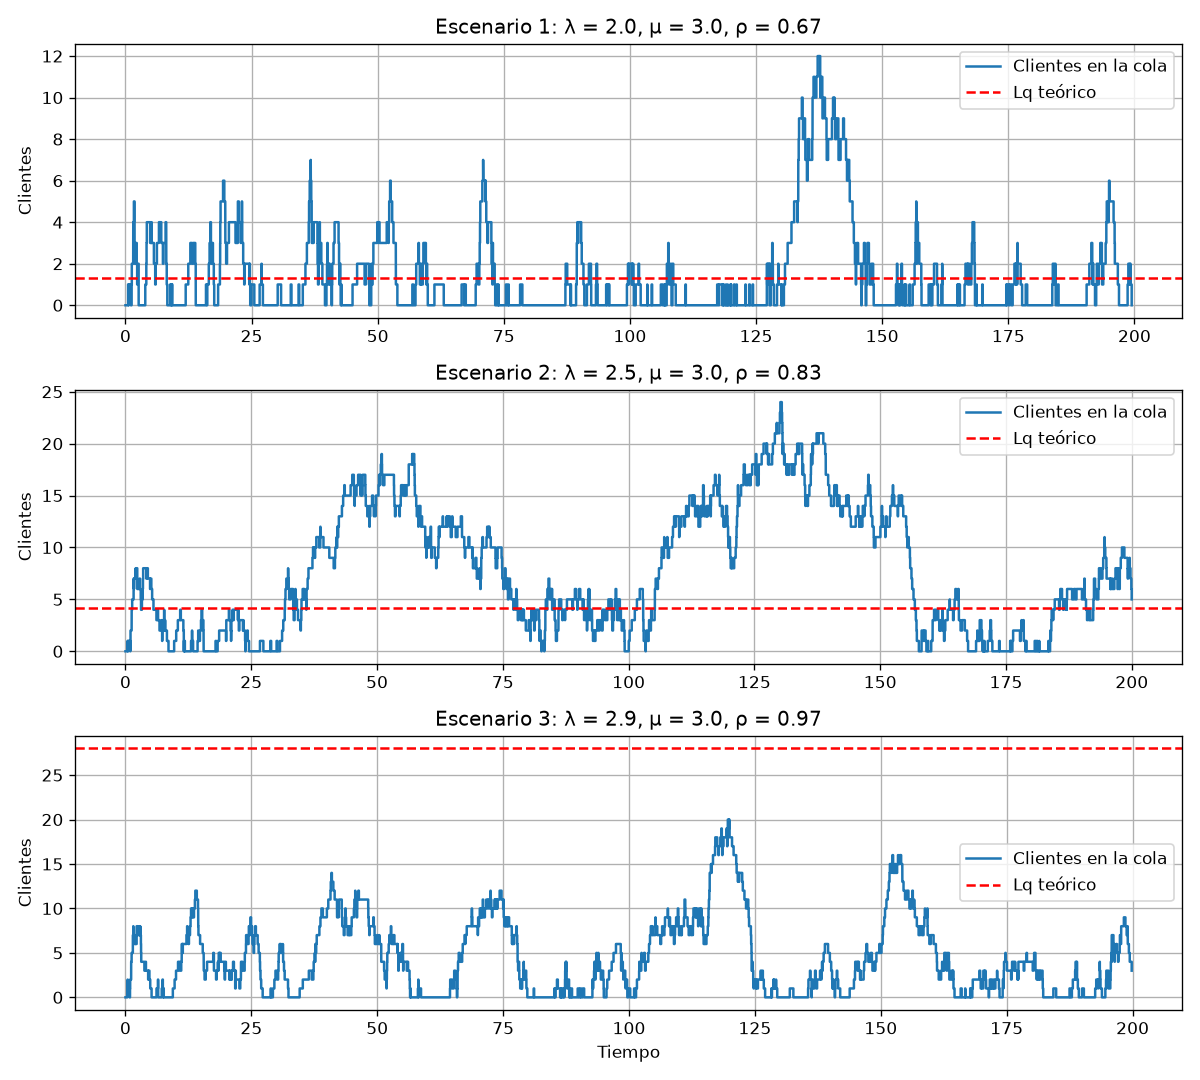
\includegraphics[width=\textwidth,height=0.53\textheight,keepaspectratio]{figures/cola_en_el_tiempo.png}
\caption{Clientes en la cola a lo largo del tiempo, un panel por escenario, con la línea
roja del valor teórico $L_q$. En el escenario 1 la cola llega como máximo a 12 clientes,
en el 2 a 24 y en el 3 a 20; en el escenario 3 queda lejos del valor teórico porque solo
se muestran las primeras 200 unidades de tiempo.}
\label{fig:cola}
\end{figure}

La Figura~\ref{fig:esperas} muestra el tiempo que esperó cada uno de los primeros 300
clientes, con la línea del valor teórico $W_q$.

\begin{figure}[H]
\centering
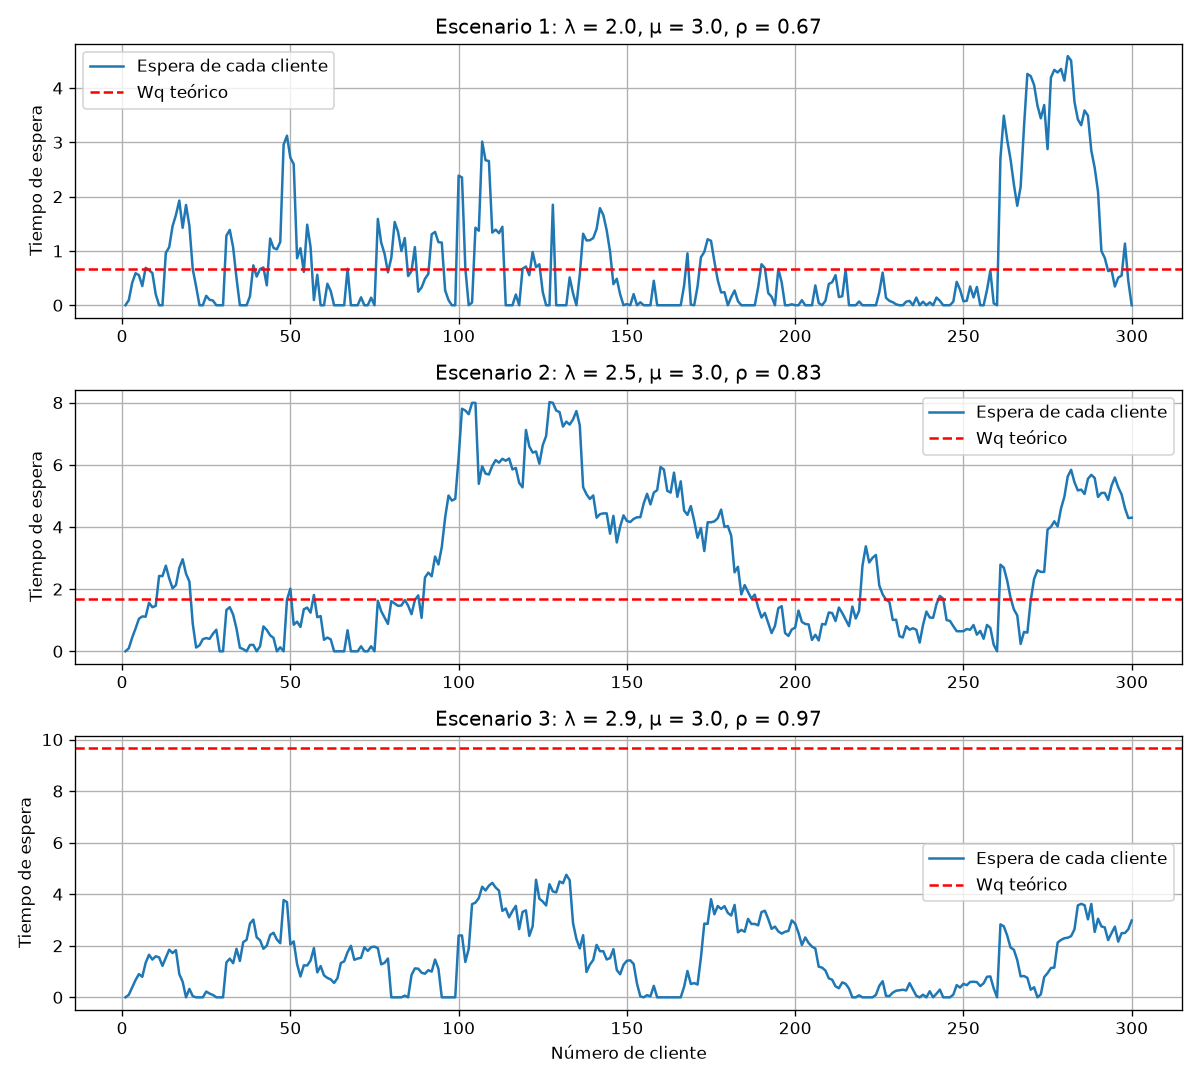
\includegraphics[width=\textwidth,height=0.46\textheight,keepaspectratio]{figures/tiempos_de_espera.png}
\caption{Tiempo de espera de cada cliente (primeros 300), un panel por escenario, con la
línea roja del valor teórico $W_q$. En el escenario 1 las esperas son pequeñas; en el
escenario 2 hay tramos largos por encima del valor teórico; y en el escenario 3 la serie
queda por debajo porque corresponde al inicio de la simulación.}
\label{fig:esperas}
\end{figure}

La Figura~\ref{fig:comparacion} compara, con barras, el valor teórico y el valor
simulado de $W_q$ y de $L_q$ en los tres escenarios.

\begin{figure}[H]
\centering
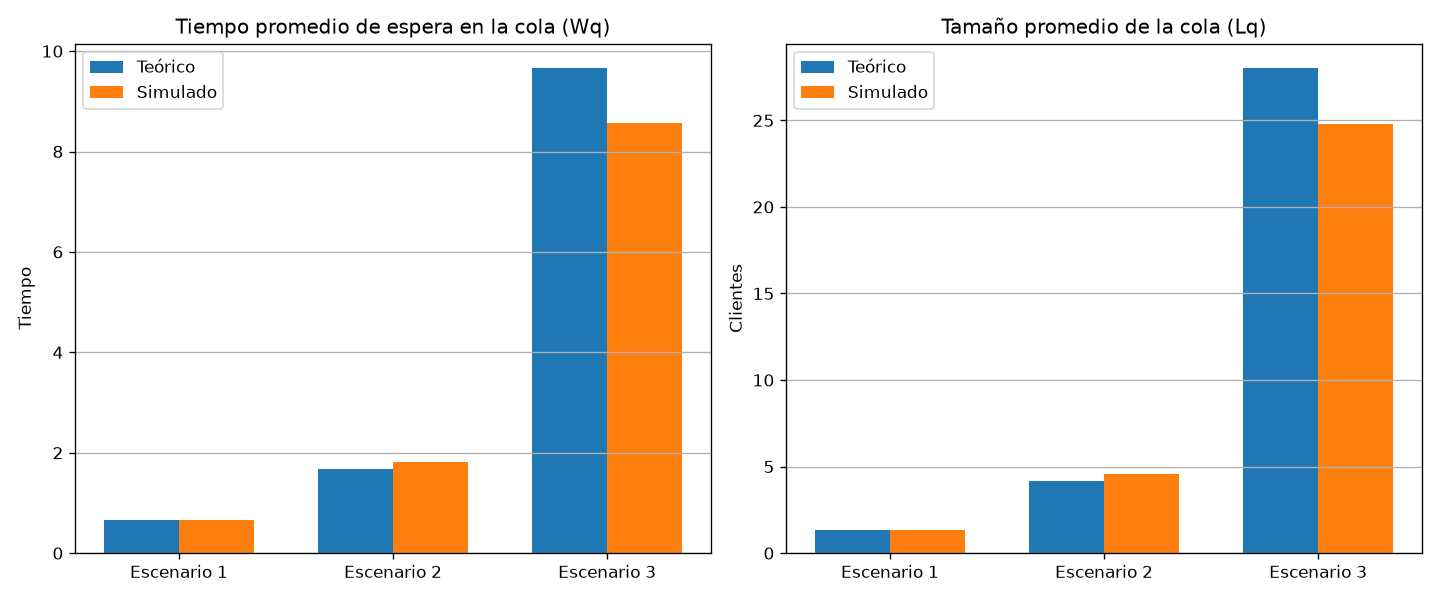
\includegraphics[width=\textwidth,height=0.22\textheight,keepaspectratio]{figures/teoria_vs_simulacion.png}
\caption{Comparación teoría -- simulación por escenario para $W_q$ (izquierda) y $L_q$
(derecha). Las barras azules son los valores teóricos y las naranjas el promedio de las
10 réplicas simuladas.}
\label{fig:comparacion}
\end{figure}

\FloatBarrier
\section{Análisis de Resultados}

En los tres escenarios el servidor trabaja siempre a $\mu = 3{,}0$ y lo único que cambia es cuántos clientes llegan: $\lambda$ sube de 2,0 a 2,9. En la Tabla~\ref{tab:comparacion} vemos que la espera en cola $W_q$ pasa de 0,67 a 1,67 y luego a 9,67, y que la cola $L_q$ pasa de 1,33 a 4,17 y luego a 28,03. Es decir, con solo un 45\,\% más de llegadas, la espera se multiplica por 14,5 y la cola por 21.

\begin{table}[h!]
\centering
\setlength{\arrayrulewidth}{0.75pt}
\arrayrulecolor{borderblue}
\renewcommand{\arraystretch}{1.3}
\small
\begin{tabular}{|c|c|c|c|c|c|c|c|c|}
\hline
\rowcolor{headerblue}
\textbf{\textcolor{white}{Esc.}} &
\textbf{\textcolor{white}{$\lambda$}} &
\textbf{\textcolor{white}{$\rho$}} &
\textbf{\textcolor{white}{$L$}} &
\textbf{\textcolor{white}{$L_q$}} &
\textbf{\textcolor{white}{$W$}} &
\textbf{\textcolor{white}{$W_q$}} &
\makecell{\textbf{\textcolor{white}{Espera}} \\ \textbf{\textcolor{white}{simulada}}} &
\makecell{\textbf{\textcolor{white}{Cola}} \\ \textbf{\textcolor{white}{simulada}}} \\ \hline
1 & 2{,}0 & 0{,}6667 & 2{,}0000 & 1{,}3333 & 1{,}0000 & 0{,}6667 & \textbf{0{,}6691} & \textbf{1{,}3350} \\ \hline
\rowcolor{rowlight}
2 & 2{,}5 & 0{,}8333 & 5{,}0000 & 4{,}1667 & 2{,}0000 & 1{,}6667 & \textbf{1{,}8141} & \textbf{4{,}5500} \\ \hline
3 & 2{,}9 & 0{,}9667 & 29{,}0000 & 28{,}0333 & 10{,}0000 & 9{,}6667 & \textbf{8{,}5730} & \textbf{24{,}8003} \\ \hline
\end{tabular}

\end{table}

La razón está en las fórmulas, donde la resta $\mu-\lambda$ aparece dividiendo. Por ejemplo, con $W = \frac{1}{\mu-\lambda}$:

\begin{itemize}
    \item Escenario 1: $\mu-\lambda = 1{,}0$, entonces $W = 1$.
    \item Escenario 2: $\mu-\lambda = 0{,}5$, entonces $W = 2$.
    \item Escenario 3: $\mu-\lambda = 0{,}1$, entonces $W = 10$.
\end{itemize}

Yo interpreto esa resta como el ``margen libre'' del servidor. Mientras es grande, el servidor se recupera rápido de cualquier racha de llegadas seguidas. Cuando es muy pequeña, casi no tiene descanso y cada acumulación de clientes tarda mucho en desaparecer. Por eso el crecimiento no es proporcional: el último tramo (de 2,5 a 2,9) pesa mucho más que los anteriores, aunque el aumento de $\lambda$ sea parecido.

\subsection{Lo que se ve en las gráficas}

\begin{figure}[H]
\centering
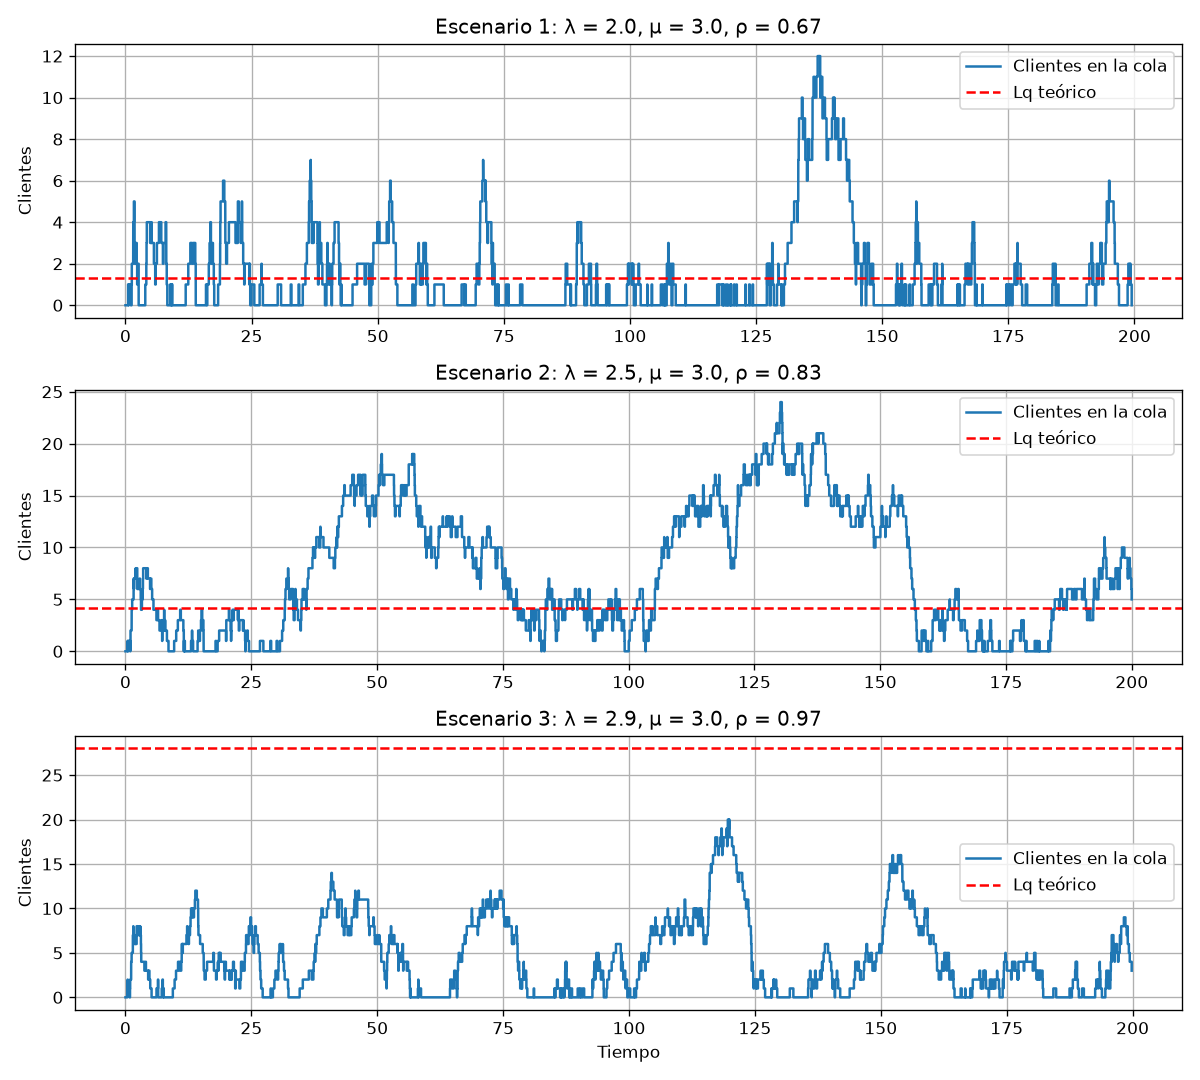
\includegraphics[width=\textwidth,height=0.43\textheight,keepaspectratio]{figures/cola_en_el_tiempo.png}

\end{figure}

\textbf{Cola en el tiempo (Figura~\ref{fig:cola}).} En el escenario 1 la línea vuelve a cero muy seguido: en las 200 unidades mostradas, la cola está vacía un poco más de la mitad del tiempo (54\,\%). Casi siempre hay entre 0 y 4 clientes, y el único momento fuera de lo normal es un pico máximo de 12 cerca del tiempo 137. En el escenario 2 el panorama cambia: la cola se vacía mucho menos (solo el 12\,\% del tiempo) y sube y baja en oleadas largas que llegan a cerca de 24 clientes. En el escenario 3 la cola llega a unos 20 clientes, pero en estas 200 unidades nunca alcanza la línea roja (28) y en promedio es incluso más corta que en el escenario 2 (unos 4 clientes contra unos 8). Eso va en contra de lo que dice la teoría; una explicación posible es que la simulación recién está empezando (se explica más abajo).

\begin{figure}[H]
\centering
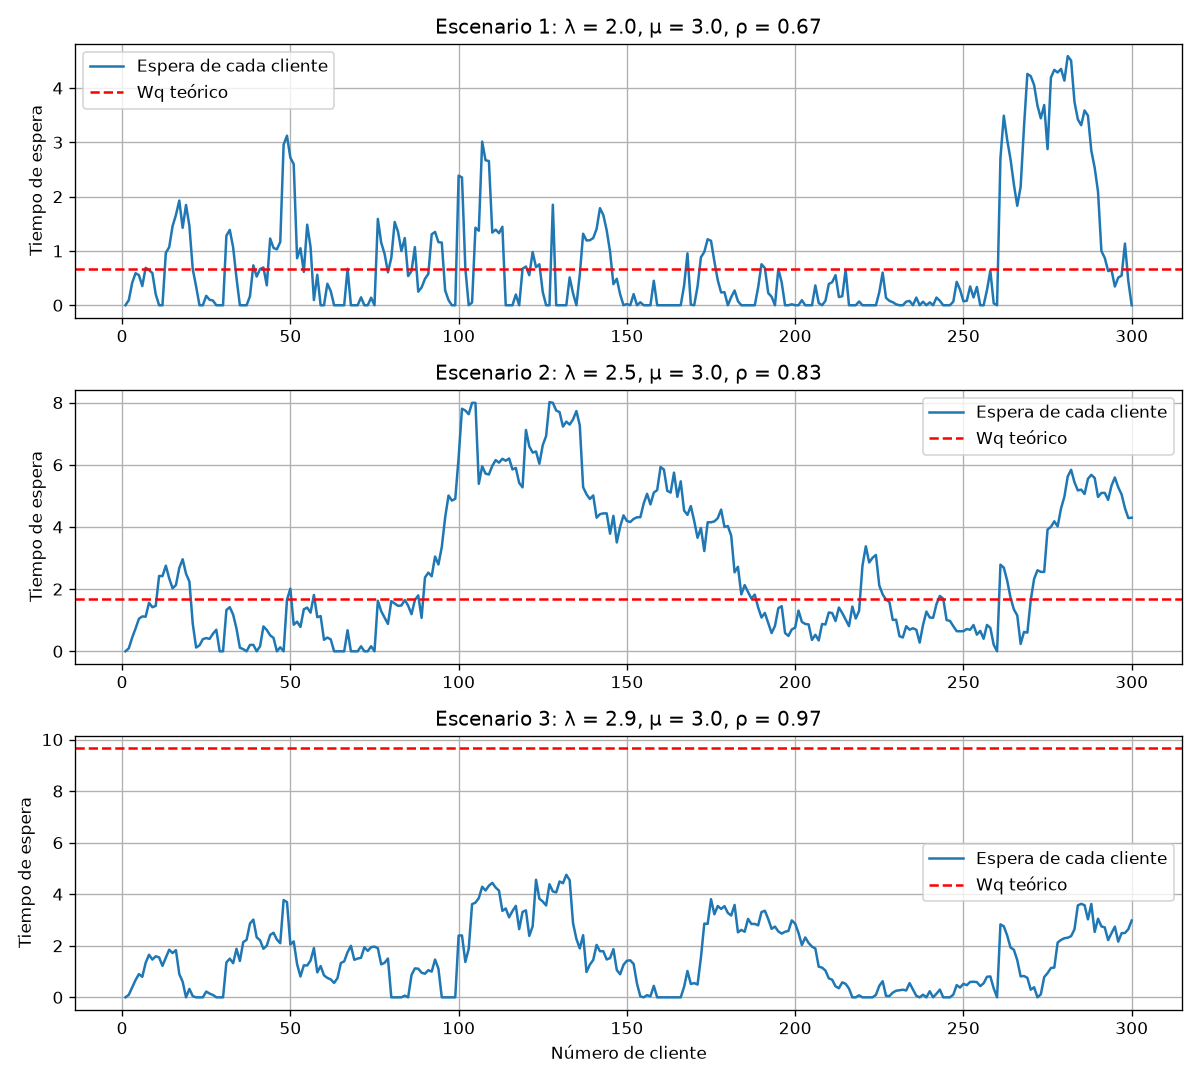
\includegraphics[width=\textwidth,height=0.4\textheight,keepaspectratio]{figures/tiempos_de_espera.png}

\end{figure}

\textbf{Espera de cada cliente (Figura~\ref{fig:esperas}).} En el escenario 1 la mayoría de los clientes espera poco, casi siempre menos de 2 unidades. Hay un grupo de clientes seguidos, cerca del número 280, pero después todo se normaliza. En el escenario 2 las esperas son más altas y duran más, pues entre los clientes 100 y 130 llegan a unas 8 unidades. Un detalle que me llamó la atención es que las esperas bajan poco a poco, porque si un cliente espera mucho, el siguiente también (ambos están en la misma fila) y la fila solo se va vaciando de a poco. Las subidas pueden ser más rápidas, por ejemplo cuando un cliente tarda mucho en ser atendido, como se ve cerca del cliente 260. En el escenario 3, en cambio, casi todos los primeros 300 clientes esperan menos de 5 unidades, muy por debajo de la línea roja. Esto es coherente con que la corrida empieza vacía y la fila todavía está creciendo hacia su tamaño normal.

\begin{figure}[H]
\centering
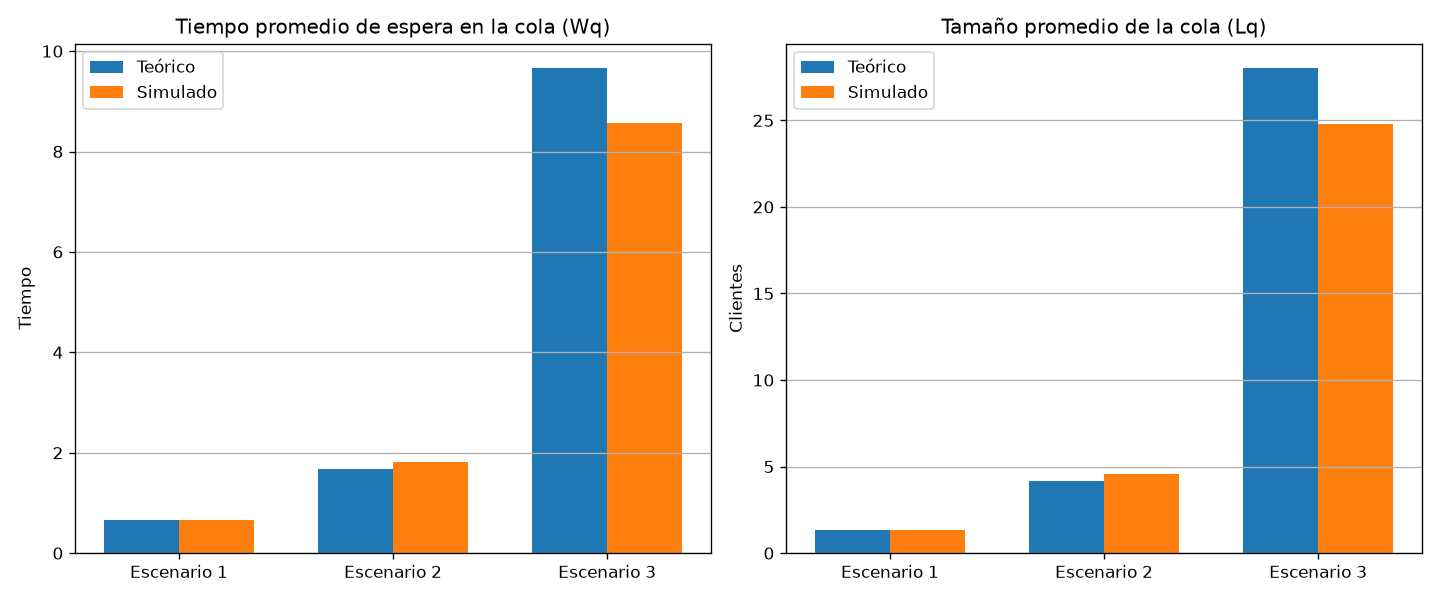
\includegraphics[width=\textwidth,height=0.22\textheight,keepaspectratio]{figures/teoria_vs_simulacion.png}

\end{figure}

\textbf{Teoría vs simulación (Figura~\ref{fig:comparacion}).} En el escenario 1 las barras azul (teórica) y naranja (simulada) son casi idénticas. En el escenario 2 la naranja queda un poco más alta y en el escenario 3 queda más baja que la azul.

\subsection{¿Por qué no coinciden exactamente?}

\begin{table}[h!]
\centering
\setlength{\arrayrulewidth}{0.75pt}
\arrayrulecolor{borderblue}
\setlength{\tabcolsep}{4pt}
\renewcommand{\arraystretch}{1.3}
\small
\begin{tabular}{|c|c|c|c|c|c|c|c|}
\hline
\rowcolor{headerblue}
\textbf{\textcolor{white}{Esc.}} &
\textbf{\textcolor{white}{Medida}} &
\makecell{\textbf{\textcolor{white}{Media}} \\ \textbf{\textcolor{white}{simulada}}} &
\makecell{\textbf{\textcolor{white}{Desv.}} \\ \textbf{\textcolor{white}{est.}}} &
\makecell{\textbf{\textcolor{white}{IC 95\,\%}}} &
\makecell{\textbf{\textcolor{white}{Valor}} \\ \textbf{\textcolor{white}{teórico}}} &
\makecell{\textbf{\textcolor{white}{\textquestiondown{}Contiene}} \\ \textbf{\textcolor{white}{al teórico?}}} &
\makecell{\textbf{\textcolor{white}{Err.}} \\ \textbf{\textcolor{white}{rel.}}} \\ \hline
1 & $W_q$ & 0{,}6691 & 0{,}0576 & $[0{,}6279;\ 0{,}7104]$ & 0{,}6667 & Sí & $+0{,}37$\,\% \\ \hline
\rowcolor{rowlight}
1 & $L_q$ & 1{,}3350 & 0{,}1243 & $[1{,}2461;\ 1{,}4240]$ & 1{,}3333 & Sí & $+0{,}13$\,\% \\ \hline
2 & $W_q$ & 1{,}8141 & 0{,}3807 & $[1{,}5418;\ 2{,}0864]$ & 1{,}6667 & Sí & $+8{,}85$\,\% \\ \hline
\rowcolor{rowlight}
2 & $L_q$ & 4{,}5500 & 0{,}9876 & $[3{,}8436;\ 5{,}2565]$ & 4{,}1667 & Sí & $+9{,}20$\,\% \\ \hline
3 & $W_q$ & 8{,}5730 & 1{,}6844 & $[7{,}3682;\ 9{,}7779]$ & 9{,}6667 & Sí & $-11{,}31$\,\% \\ \hline
\rowcolor{rowlight}
3 & $L_q$ & 24{,}8003 & 5{,}0023 & $[21{,}2221;\ 28{,}3785]$ & 28{,}0333 & Sí & $-11{,}53$\,\% \\ \hline
\end{tabular}

\end{table}

En la Tabla~\ref{tab:intervalos} se ve que la diferencia en $W_q$ es mínima en el escenario 1 ($+0{,}37$\,\%), de cerca de $+9$\,\% en el escenario 2 y de cerca de $-11$\,\% en el escenario 3. Veo dos explicaciones posibles:

\begin{itemize}
    \item \textbf{El azar:} Cada réplica usa números aleatorios distintos, así que ninguna da exactamente el valor teórico. Además, cuanto más cargado está el sistema, más cambian los resultados de una réplica a otra: la desviación estándar de $W_q$ sube de 0,058 a 0,381 y a 1,684 entre los escenarios 1, 2 y 3.
    \item \textbf{El inicio vacío:} La simulación arranca sin clientes, pero la teoría describe el sistema ya estabilizado. Al principio la cola es más corta de lo normal y eso baja los promedios, esto se nota sobre todo en el escenario 3, porque con $\rho = 0{,}967$ el sistema tarda mucho en llenarse. Por eso las gráficas de ese escenario quedan por debajo de la línea roja.
\end{itemize}

Como el escenario 2 queda por encima de la teoría y el 3 por debajo, el azar parece tener un papel importante. Para separarlas habría que descartar el tramo inicial de cada corrida o usar más réplicas.

\subsection{Los intervalos de confianza}

En los seis casos de la Tabla~\ref{tab:intervalos}, el valor teórico cae dentro del intervalo de confianza al 95\,\%. Dicho de forma simple: con lo que simulamos, \textbf{no hay evidencia de que la simulación esté mal}, porque las diferencias son compatibles con el azar (pero eso no significa que sea exacta). En el escenario 3 los intervalos son anchos (por ejemplo, el de $W_q$ va de 7,37 a 9,78), así que parte de la razón por la que la teoría cabe es que el intervalo deja mucho margen; con más réplicas se estrecharía y la comparación sería más exigente.

\subsection{¿Por qué hacer varias corridas?}

Logré entender que el resultado cambia mucho de una corrida a otra. En el escenario 3 la desviación de $W_q$ entre réplicas es 1,68, cerca del 20\,\% de la media simulada (8,57). Una sola corrida podría salir bastante más alta o más baja que el valor real y llevarnos a una conclusión equivocada. En el escenario 1 la desviación entre réplicas es solo 0,058, cerca del 9\,\% de la media, y una corrida sola ya sería bastante confiable. Por eso hicimos 10 réplicas por escenario: el promedio de varias corridas es mucho más seguro que una sola.

\FloatBarrier
\section{Preguntas de Control}

\begin{enumerate}
    \item \textbf{\textquestiondown{}Qué representa el modelo M/M/1?}
    \par El modelo $M/M/1$ representa una fila de espera con un solo servidor que atiende a los clientes uno por uno \cite{smith2024}. Los tiempos entre llegadas y los tiempos de atención son aleatorios y siguen una distribución exponencial \cite{smith2024, heather2026}. Los clientes forman una sola fila sin límite de espacio, se atienden en orden de llegada (FIFO) y salen del sistema al terminar \cite{smith2024}.

    \item \textbf{\textquestiondown{}Qué representan $\lambda$ y $\mu$?}
    \par $\lambda$ es la rapidez con la que llegan los clientes, osea cuántos llegan por unidad de tiempo \cite{smith2024}. $\mu$ es la rapidez con la que el servidor atiende, osea cuántos clientes puede atender por unidad de tiempo \cite{smith2024, heather2026}. Juntos indican qué tan ocupado estará el sistema \cite{smith2024}.

    \item \textbf{\textquestiondown{}Por qué debe cumplirse $\lambda < \mu$ para que el sistema sea estable?}
    \par Porque el servidor debe atender clientes más rápido de lo que llegan \cite{smith2024}. Si es así, la fila no crece sin parar y el sistema se mantiene en equilibrio \cite{smith2024}. En ese caso la utilización es menor a uno ($\rho < 1$), es decir, el servidor tiene tiempo libre \cite{smith2024}.

    \item \textbf{\textquestiondown{}Qué significa la utilización $\rho$?}
    \par La utilización $\rho$ representa la proporción del tiempo en que el servidor está ocupado atendiendo entidades \cite{smith2024, heather2026}. Para un servidor único se calcula como $\rho = \lambda/\mu$ \cite{smith2024}. Un valor alto de $\rho$ indica mayor carga sobre el recurso y mayor congestión del sistema \cite{smith2024}.

    \item \textbf{\textquestiondown{}Cuál es la diferencia entre $W$ y $W_q$?}
    \par $W_q$ es el tiempo promedio que una entidad pasa únicamente esperando en la cola antes de ser atendida \cite{smith2024, heather2026}. $W$ es el tiempo promedio total en el sistema, que incluye la espera en cola y el tiempo de servicio \cite{smith2024, heather2026}.

    \item \textbf{\textquestiondown{}Cuál es la diferencia entre $L$ y $L_q$?}
    \par $L_q$ es el número promedio, ponderado en el tiempo, de entidades que esperan en la cola \cite{smith2024, heather2026}. $L$ es el número promedio total de entidades en el sistema, es decir, las que esperan más las que reciben servicio \cite{smith2024, heather2026}.

    \item \textbf{\textquestiondown{}Por qué SimPy utiliza una distribución exponencial para generar los tiempos?}
    \par En los modelos de colas simulados con SimPy se usa la distribución exponencial por su propiedad de ``falta de memoria'' (\emph{memoryless property}) \cite{baxter2024, smith2024}. Esta propiedad simplifica la modelación de llegadas de Poisson y de tiempos de servicio independientes \cite{heather2026, smith2024}. Además, permite verificar la simulación comparándola con las soluciones analíticas teóricas de colas $M/M/s$ \cite{heather2026, smith2024}.

    \item \textbf{\textquestiondown{}Qué sucede con la cola cuando $\lambda$ se aproxima a $\mu$?}
    \par Cuando $\lambda$ se aproxima a $\mu$, la utilización $\rho$ tiende a $1$ \cite{smith2024}. Esto genera un crecimiento desproporcionado de la congestión y de la acumulación de entidades \cite{smith2024}. Como resultado, tanto la longitud promedio de la cola ($L_q$) como el tiempo medio de espera ($W_q$) aumentan drásticamente, tendiendo al infinito \cite{smith2024}.

    \item \textbf{\textquestiondown{}Por qué los resultados simulados pueden ser diferentes de los resultados teóricos?}
    \par Porque la simulación usa números aleatorios, y por eso cada corrida da resultados un poco distintos \cite{smith2024}. Además, la simulación empieza con el sistema vacío, y eso afecta los primeros resultados mientras el sistema se estabiliza (\emph{warm-up}) \cite{smith2024, heather2026}. La teoría da el valor exacto a muy largo plazo, mientras que la simulación solo lo estima con un número limitado de corridas \cite{smith2024, heather2026}.

    \item \textbf{\textquestiondown{}Qué ocurriría si $\lambda$ fuera mayor que $\mu$?}
    \par Si $\lambda > \mu$, llegan más clientes de los que el servidor puede atender, y el sistema se vuelve inestable ($\rho > 1$) \cite{smith2024}. Como el servidor no alcanza a atenderlos a tiempo, la fila crece sin parar \cite{smith2024}. El sistema nunca llega a un equilibrio, y las fórmulas de $L$, $L_q$, $W$ y $W_q$ dejan de aplicarse \cite{smith2024}.
\end{enumerate}

\FloatBarrier
\section{Conclusiones}

\begin{itemize}
    \item Se logró implementar el sistema M/M/1 con SimPy, con llegadas de clientes,
    una cola y un único servidor, y se pudo ejecutar los tres escenarios con el mismo
    programa cambiando solo $\lambda$.
    \item Las métricas teóricas ($\rho$, $L$, $L_q$, $W$ y $W_q$) mostraron que el
    sistema se vuelve muy sensible cuando $\lambda$ se acerca a $\mu$: al pasar de
    $\rho = 0{,}667$ a $\rho = 0{,}967$ la espera teórica sube de 0,67 a 9,67 unidades
    de tiempo, aunque la tasa de llegadas solo aumentó de 2,0 a 2,9.
    \item La simulación confirmó lo esperado: a mayor $\lambda$, más espera y colas más
    largas. Los valores simulados quedaron cerca de los teóricos, y en los tres
    escenarios la teoría cayó dentro del intervalo de confianza del 95\,\%.
    \item Las diferencias que aparecen se explican por el azar y porque la simulación
    arranca con el sistema vacío, algo que pesa más en el escenario 3. Por eso conviene
    repetir la simulación varias veces y no confiar en una sola corrida.
\end{itemize}

\section{Declaración de uso de Inteligencia Artificial}

En este trabajo se usaron herramientas de inteligencia artificial como apoyo, no como
sustituto del trabajo propio. Primero se muestra un prompt representativo de la forma en
que se usó la herramienta y, a continuación, la justificación de su uso.

\subsection{Prompt utilizado}

El estudiante partió siempre de contenido ya elaborado (informe, código y resultados
propios) y pidió mejorarlo, no generarlo desde cero. El siguiente prompt resume la
instrucción general empleada (es representativo, no una transcripción literal de todas
las interacciones):

\begin{quote}
\small
\textit{Te comparto mi informe de la práctica 003 (simulación de un sistema M/M/1 con
SimPy) escrito en \LaTeX{} para Overleaf, junto con la guía del docente. Ya tengo
redactados el fundamento teórico, las tablas de resultados y las gráficas, y ya ejecuté
mi programa. Necesito que me ayudes a \textbf{mejorar} lo que ya tengo, no a hacerlo
desde cero:}

\textit{1. Redacción: revisa mi análisis de resultados y propón una versión con
lenguaje más claro y natural, sin cambiar mis números.}

\textit{2. Formato: corrige mi código \LaTeX{} para que las figuras y las tablas no se
superpongan con el texto y para que las citas salgan en estilo IEEE usando mi archivo
\texttt{referencias.bib}.}

\textit{3. Fórmulas y modelo matemático: verifica que $\rho$, $L$, $L_q$, $W$ y $W_q$ y
la condición $\lambda < \mu$ estén bien según la guía, y avísame si encuentras errores.}

\textit{4. Estructura del código: dime si mi organización en modelo, vista y
controlador es adecuada y qué mejorarías.}

\textit{Reglas: no inventes datos ni referencias. Las respuestas de las preguntas de
control salen del cuaderno de NotebookLM compartido por el docente; solo ayúdame a
simplificar su redacción. Si algo no puedes verificar, dímelo.}
\end{quote}

\subsection{Justificación del uso}

\textbf{Herramientas utilizadas.}

\begin{itemize}
    \item \textbf{Claude Sonnet 5.5} (Anthropic), mediante la aplicación web claude.ai.
    \item \textbf{NotebookLM} (Google), con el cuaderno de documentos compartido por el
    docente.
\end{itemize}

\textbf{Apoyo recibido de Claude.}

\begin{itemize}
    \item \textbf{Redacción:} mejora de la claridad de los textos, simplificación de las
    respuestas de las preguntas de control y borrador del análisis de resultados a
    partir de las tablas y gráficas obtenidas.
    \item \textbf{Formato:} escritura y corrección del código \LaTeX{} en Overleaf,
    incluida la ubicación de figuras y tablas y el estilo de las citas.
    \item \textbf{Indagación de fórmulas y modelo matemático:} revisión de las fórmulas
    de $\rho$, $L$, $L_q$, $W$ y $W_q$ y de la condición de estabilidad $\lambda < \mu$,
    contrastadas con la guía de la práctica.
    \item \textbf{Estructura del código:} orientación sobre la organización del programa
    en modelo, vista y controlador.
\end{itemize}

\textbf{Lo que no se hizo con IA.}

\begin{itemize}
    \item La información de las \textbf{preguntas de control} se obtuvo del cuaderno de
    NotebookLM compartido por el docente, a partir de sus documentos cargados. Claude
    solo ayudó a reformular esas respuestas con un lenguaje más sencillo y a pasarlas
    a \LaTeX{}.
    \item El archivo de referencias (\texttt{referencias.bib}) se generó a partir de
    ese mismo cuaderno.
    \item Los resultados numéricos, las tablas y las gráficas provienen de la ejecución
    del programa por parte del estudiante.
\end{itemize}

\textbf{Alcance y verificación:} La inteligencia artificial \textbf{no se usó para
elaborar el informe completo}. El estudiante revisó los textos, comprobó que los valores
y comentarios coincidieran con sus propios resultados y es responsable del contenido
final. Dado que las herramientas de IA pueden cometer errores, las respuestas y las
referencias se contrastaron con la guía de la práctica y con las fuentes del cuaderno
del docente.

\section{Bibliografía}

\bibliographystyle{IEEEtran}
\bibliography{referencias}

\end{document}
